\documentclass{beamer}

\usepackage{hyperref}
\usepackage{graphicx}
\usepackage{tikz}
\usetikzlibrary{calc}

\newcommand{\NH}{\text{NH}}
\newcommand{\RG}{\text{RG}}

\title{Measuring the Price of Anarchy in Critical Care Unit Interactions}
\author{Vincent Knight and Izabella Komenda}
\date{2014-07-25}

\setbeamertemplate{navigation symbols}{}

\begin{document}

\frame{
\begin{center}
\href{}{+Vincent.Knight}\\
\href{}{@drvinceknight}\\
\url{www.vincent-knight.com}\\
\url{drvinceknight.github.io/Talks}\\
\vspace{1cm}
\href{}{@IzabelaKomenda}
\end{center}
}

\frame{
    \Huge
    \[
        \begin{pmatrix}
        (2,2)&(5,0)\\
        (0,5)&(4,4)
        \end{pmatrix}
    \]
}

\frame{
    \begin{center}
        \includegraphics[width=.8\textwidth]{./Images/PoA_Healthcare.pdf}
    \end{center}
}

\frame{
    \begin{center}
        {\Huge What about the controllers?}\\
        \vspace{1cm}
    \end{center}
        \pause
        S. Deo and I. Gurvich. \textbf{Centralized vs. Decentralized Ambulance Diversion: A Network Perspective.} \textit{Management Science}, 57(7):1300–1319, May 2011.
}

\frame{
    \begin{center}
        [INCLUDE ANY PLOT FROM PAPER WITH IZA]
    \end{center}
    \pause
    \textbf{Mathematical modelling of patient flows to predict critical care capacity required following the merger of two District General Hospitals into one.}, \textit{Submitted to Anaesthesia}
}

\frame{
\begin{center}
    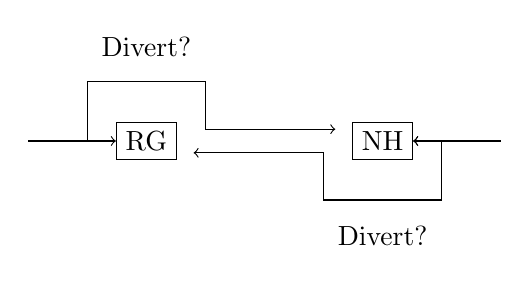
\begin{tikzpicture}[scale=1.5]
        \node (A) at (0,0) [draw] {RG};
        \node (B) at (2,0) [draw] {NH};
        \draw [->] (-1,0) -- (A);
        \draw [->] (3,0) -- (B);
        \draw [->] (-1,0) -- ($(A)+(-.5,0)$) -- ($(A)+(-.5,.5)$) -- ($(A)+(.5,.5)$) -- ($(A)+(.5,.1)$) -- ($(B)+(-.4,.1)$);
        \draw [->] (3,0) -- ($(B)+(.5,0)$) -- ($(B)+(.5,-.5)$) -- ($(B)+(-.5,-.5)$) -- ($(B)+(-.5,-.1)$) -- ($(A)+(.4,-.1)$);
        \draw [->] (3,0) -- (B);
        \node at ($(A) + (0,.8)$) {Divert?};
        \node at ($(B) + (0,-.8)$) {Divert?};
    \end{tikzpicture}
\end{center}
}

\frame{
\begin{center}
    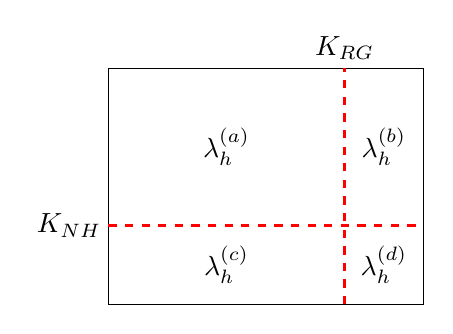
\begin{tikzpicture}
        \draw  (0,0) rectangle (4,3);
        \draw [dashed, red, thick] (0,1) -- (4,1);
        \draw [dashed, red, thick] (3,0) -- (3,3);
        \node at (-.5,1) {$K_{\NH}$};
        \node at (3,3.25) {$K_{\RG}$};
        \node at (1.5,2) {$\lambda_{h}^{(a)}$};
        \node at (3.5,2) {$\lambda_{h}^{(b)}$};
        \node at (1.5,.5) {$\lambda_{h}^{(c)}$};
        \node at (3.5,.5) {$\lambda_{h}^{(d)}$};
    \end{tikzpicture}
\end{center}
}

\end{document}
